%%%%%%%%%%%%%%%%%%%%%%%%
%
% $Autor: Daanyaal Parvaize, Kreetika Mohanta, Keerti Belmane$
% $Datum: 2025-06-11 20:48:02Z $
% $Pfad: BA25-02-Time-Series/report/Contents/en/DocumentationDeveloper.tex
% $Version: 4621 $
%
% !TeX encoding = utf8
% !TeX root = Rename
%
%%%%%%%%%%%%%%%%%%%%%%%%

\chapter{Developer Documentation}

\section{Introduction}

This chapter documents the complete development framework for the storm wind speed forecasting project using ARIMA and LSTM models.  
It is intended to serve as a reference for developers maintaining or extending the system, providing a comprehensive understanding of the architecture, workflows, coding standards, and operational guidelines.  

The project employs a modular approach to machine learning pipeline implementation, emphasizing robustness, flexibility, and clarity.  
Special attention is given to parameter management, error handling, and reproducibility.

\section{Development Idea and Objectives}

The primary objective of this project is to create an extensible and maintainable machine learning training pipeline that:

\begin{itemize}
	\item Automates data ingestion and preprocessing.
	\item Supports multiple model architectures (ARIMA, LSTM) with clearly separated workflows.
	\item Validates all configurations to prevent runtime errors.
	\item Provides fallback mechanisms for data unavailability.
	\item Ensures consistent saving and documentation of outputs.
	\item Facilitates clear logging and error reporting to ease debugging.
	\item Encourages code readability and modularity for collaborative development.
\end{itemize}

This architecture allows future incorporation of new forecasting models with minimal impact on the existing codebase.

\section{System Architecture and Flowcharts}

The system workflow can be summarized in three main phases, each representing a critical stage in the development and operation of the forecasting system. The flowchart below visually depicts these phases and their sequential dependencies:

\begin{center}
	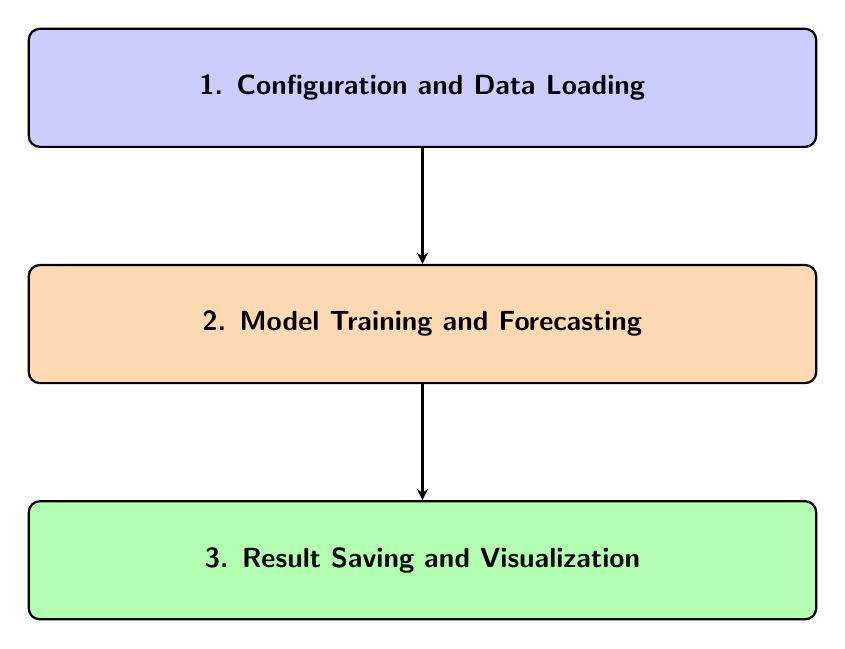
\begin{tikzpicture}[node distance=3cm]
		
		% Define basic styles
		\tikzset{
			phase/.style={
				rectangle, draw=black, thick, rounded corners, 
				minimum width=10cm, minimum height=1.5cm,
				fill=blue!20, font=\sffamily\bfseries
			},
			arrow/.style={
				thick, ->, >=stealth
			}
		}
		
		% Nodes
		\node[phase] (config) {1. \textbf{Configuration and Data Loading}};
		\node[phase, fill=orange!30, below of=config] (training) {2. \textbf{Model Training and Forecasting}};
		\node[phase, fill=green!30, below of=training] (results) {3. \textbf{Result Saving and Visualization}};
		
		% Arrows
		\draw[arrow] (config) -- (training);
		\draw[arrow] (training) -- (results);
		
	\end{tikzpicture}
\end{center}

\subsection*{1. Configuration and Data Loading}

This initial phase lays the foundation for the entire forecasting pipeline. It includes the following key activities:

\begin{itemize}
	\item \textbf{Parameter Configuration:} System parameters such as data source paths, model hyperparameters (e.g., ARIMA order or LSTM architecture), and environment variables are initialized. Parameter handling modules validate these inputs to ensure correctness and provide default fallbacks to prevent runtime failures.
	\item \textbf{Data Ingestion:} Raw data is loaded from persistent storage or external sources. This involves robust file handling mechanisms to support multiple data formats (CSV, JSON, databases), and error handling to capture and report missing or corrupted files.
	\item \textbf{Data Preprocessing:} The ingested data undergoes cleaning, normalization, and transformation steps. Preprocessing modules detect outliers, handle missing values, and convert timestamps for time series alignment. These operations ensure the data integrity required for accurate forecasting.
	\item \textbf{Logging and Messaging:} Throughout this phase, logging systems capture detailed messages for debugging and audit purposes, while user-facing messages inform the operator of progress or issues encountered.
\end{itemize}

\subsection*{2. Model Training and Forecasting}

This core phase involves the execution of machine learning algorithms to generate predictive insights:

\begin{itemize}
	\item \textbf{Training Module:} Depending on the configured algorithm (e.g., ARIMA, LSTM), the system initializes and trains the forecasting model on historical data. The module supports parameter tuning and early stopping criteria to optimize model performance.
	\item \textbf{Forecast Generation:} After training, the model forecasts future hurricane intensities for specified time horizons. The pipeline supports batch and incremental predictions to accommodate various use cases.
	\item \textbf{Error Handling and Recovery:} This phase is equipped with error detection routines to manage issues such as convergence failures or incompatible data shapes, ensuring the system can gracefully recover or notify developers.
	\item \textbf{Modularity and Extensibility:} The architecture follows a modular design, allowing easy integration of additional forecasting models or updated algorithms without affecting other components.
\end{itemize}

\subsection*{3. Result Saving and Visualization}

The final phase ensures that model outputs are persisted and accessible for stakeholders:

\begin{itemize}
	\item \textbf{Persistence Layer:} Forecast results, including point predictions and confidence intervals, are saved in structured formats (e.g., databases, CSV files) for downstream analysis or archival.
	\item \textbf{Visualization Module:} Interactive dashboards and static plots are generated to visually communicate forecast trends and model performance metrics. This supports informed decision-making by researchers and disaster management teams.
	\item \textbf{Reporting and Exporting:} The system supports export functionality for sharing results in common formats (PDF, Excel), enhancing collaboration across departments.
	\item \textbf{Notification System:} Optionally, automated alerts can be sent based on threshold conditions (e.g., forecasted hurricane intensity exceeds a critical level), enabling proactive responses.
\end{itemize}

\subsection*{Architectural Overview}

The system employs a layered architecture with clear separation of concerns:

\begin{itemize}
	\item \textbf{Input Layer:} Handles user inputs, configuration files, and raw data ingestion.
	\item \textbf{Processing Layer:} Contains the data preprocessing and model training pipelines, encapsulated into reusable and testable modules.
	\item \textbf{Output Layer:} Manages result persistence, visualization generation, and user notifications.
\end{itemize}

This architecture promotes maintainability, scalability, and ease of debugging by isolating functionality and enforcing strict interfaces between components. The use of robust parameter and error handling mechanisms throughout the system ensures operational reliability and user confidence.



\subsection{Overall Pipeline Flowchart}

\begin{center}
	\resizebox{\textwidth}{!}{ % Scale to fit page width
		\begin{tikzpicture}[
			node distance=1.8cm and 2cm,
			every node/.style={
				rectangle, draw=black!70, thick, rounded corners,
				minimum height=1cm,
				text width=6cm, 
				align=center,
				font=\small,
				fill=blue!10
			},
			decision/.style={
				diamond, draw=red!80, thick, fill=red!20,
				text width=4.8cm, align=center,
				inner sep=0pt, font=\small\bfseries,
				aspect=2
			},
			->, >=stealth', thick
			]
			
			% Nodes
			\node (start) {Start};
			
			\node (loadconfig) [below=of start] {Load and validate configuration file\\ \footnotesize (Parameters, model choices, file paths)};
			
			\node (loaddata) [below=of loadconfig] {Load storm wind speed data\\ \footnotesize (From CSV/Kaggle dataset)};
			
			\node (datacheck) [decision, below=1.5cm of loaddata] {Is data valid and sufficient?\\ \footnotesize (Data cleaning checks for outliers, anomalies)};
			
			\node (yesnode) [left=1.6cm of datacheck, font=\bfseries\small] {Yes};
			\node (nonode) [right=1.6cm of datacheck, font=\bfseries\small] {No};
			
			\node (gendata) [right=2.4cm of nonode] {Generate default synthetic data\\ \footnotesize (Fallback data for testing)};
			
			\node (choosemodel) [below=2.2cm of datacheck] {Select model type\\ \footnotesize (ARIMA or LSTM)};
			
			\node (trainarima) [below left=3cm and 2cm of choosemodel, fill=orange!20] {Train ARIMA model\\ \footnotesize (Statistical training via ModelCard)};
			
			\node (trainlstm) [below right=3cm and 2cm of choosemodel, fill=orange!20] {Train LSTM model\\ \footnotesize (Deep learning via DomainTools)};
			
			\node (saveoutput) [below=5.5cm of choosemodel, xshift=1.5cm, fill=green!20] {Save trained model, forecast CSV, and plots\\ \footnotesize (Results saved via DomainKnowledge module)};
			
			\node (end) [below=of saveoutput] {End};
			
			% Connections
			\draw (start) -- (loadconfig);
			\draw (loadconfig) -- (loaddata);
			\draw (loaddata) -- (datacheck);
			
			\draw (datacheck.west) -- (yesnode.east);
			\draw (yesnode) |- (choosemodel);
			
			\draw (datacheck.east) -- (nonode.west);
			\draw (nonode) -- (gendata);
			\draw (gendata) |- (choosemodel);
			
			\draw (choosemodel) -- node[above left] {ARIMA} (trainarima);
			\draw (choosemodel) -- node[above right] {LSTM} (trainlstm);
			
			\draw (trainarima) |- (saveoutput);
			\draw (trainlstm) |- (saveoutput);
			
			\draw (saveoutput) -- (end);
		\end{tikzpicture}
	}
\end{center}





\subsubsection*{Detailed Explanation}

The above pipeline encapsulates the entire lifecycle of the forecasting system, divided into logical, manageable steps:

\paragraph{Start to Configuration Validation}  
The pipeline begins by loading and validating the configuration file, a key responsibility of the \texttt{DocumentationDeveloper} module. This file dictates model parameters (such as ARIMA order or LSTM architecture), data file locations, and runtime flags. Rigorous validation here prevents cascading errors downstream by ensuring input integrity.

\paragraph{Data Loading and Validation}  
Data ingestion is performed next, primarily by the \texttt{DataMining} module, which reads storm wind speed data from sources like NOAA or Kaggle datasets. Post ingestion, the \texttt{DomainTools} module’s data cleaning components validate the dataset’s completeness and statistical adequacy, detecting missing values or anomalies critical for accurate model training.

\paragraph{Synthetic Data Generation as Fallback}  
If the raw data is found invalid or insufficient, a synthetic data generator activates to produce default or simulated datasets. This enables pipeline testing and continuous integration workflows without blocking on external data availability.

\paragraph{Model Selection and Training}  
Following data validation, the system proceeds to model selection. It supports both statistical models (ARIMA) and machine learning models (LSTM), allowing flexible forecasting approaches tailored to specific research or operational needs.  
- The ARIMA model training, described in the \texttt{ModelCard} file, fits time series parameters using autoregressive and moving average components, optimized with model order selection heuristics.  
- The LSTM model training, within \texttt{DomainTools}, leverages recurrent neural networks to capture temporal dependencies in the data, trained with backpropagation through time and regularization techniques.

\paragraph{Result Saving and Visualization}  
Once training completes, the pipeline saves the resulting models, forecasts, and corresponding visualization plots for further analysis and reporting. These outputs support scientific publication and operational decision-making. The \texttt{DomainKnowledge} module handles saving to standard formats and generating interactive or static visualizations, ensuring traceability and reproducibility.

\paragraph{End of Pipeline}  
The process concludes cleanly, ready for subsequent executions or integration into larger decision support systems.


This pipeline design ensures modularity, robustness, and extensibility. Each step can be individually developed, tested, and maintained, with clear data and control flow between modules — crucial for collaborative development and scalable maintenance.





\subsection{ARIMA and LSTM Training Flowcharts with Explanations}

\textbf{Step-by-step explanation of ARIMA Model Training:}

\begin{itemize}
	\item \textbf{Start ARIMA Training:} This step signals the beginning of the ARIMA modeling process.
	\item \textbf{Extract ARIMA hyperparameters (p, d, q):}
	\begin{itemize}
		\item \(p\): number of past observations (lags) used for prediction.
		\item \(d\): number of times the data needs to be differenced to make it stationary.
		\item \(q\): number of lagged forecast errors included in the model.
	\end{itemize}
	\item \textbf{Validate parameters for consistency:} Ensure that the parameters are logical and not overfitted or unstable.
	\item \textbf{Fit ARIMA model to wind speed series:} Train the ARIMA model on historical wind speed data to capture trends and patterns.
	\item \textbf{Forecast next 10 time steps:} Use the trained model to predict the wind speed values for the next 10 periods.
	\item \textbf{Save trained ARIMA model to disk:} Save the model for future use so you don’t need to retrain.
	\item \textbf{Save forecasted values as CSV:} Store the predicted wind speed values in a .csv file for later use or analysis.
	\item \textbf{Plot historical and forecasted data:} Visualize both past and predicted values in one graph for better understanding.
	\item \textbf{Save plot image:} Export the visual plot as an image file for reports or presentations.
	\item \textbf{End ARIMA Training:} Finish the entire ARIMA pipeline.
\end{itemize}

\begin{center}
	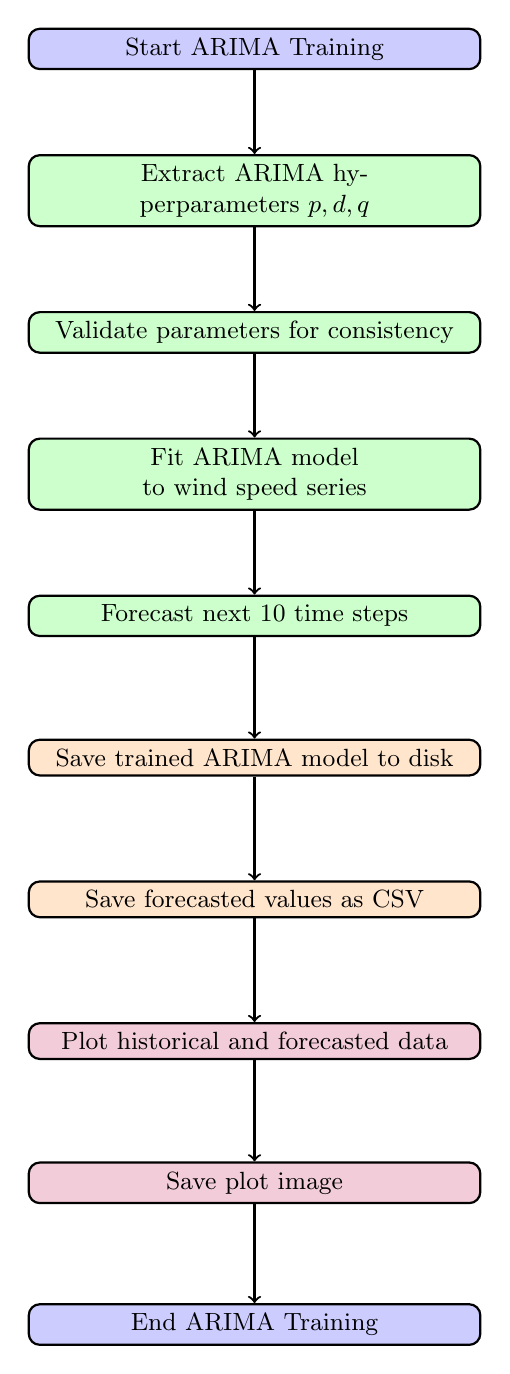
\begin{tikzpicture}[node distance=1.8cm, every node/.style={rectangle, draw, rounded corners, text width=5.5cm, align=center, font=\small}, ->, thick]
		\tikzstyle{startend} = [fill=blue!20]
		\tikzstyle{process} = [fill=green!20]
		\tikzstyle{save} = [fill=orange!20]
		\tikzstyle{plot} = [fill=purple!20]
		
		\node[startend] (start) {Start ARIMA Training};
		\node[process] (extract) [below of=start] {Extract ARIMA hyperparameters \(p,d,q\)};
		\node[process] (validate) [below of=extract] {Validate parameters for consistency};
		\node[process] (fit) [below of=validate] {Fit ARIMA model to wind speed series};
		\node[process] (forecast) [below of=fit] {Forecast next 10 time steps};
		\node[save] (savemodel) [below of=forecast] {Save trained ARIMA model to disk};
		\node[save] (saveforecast) [below of=savemodel] {Save forecasted values as CSV};
		\node[plot] (plot) [below of=saveforecast] {Plot historical and forecasted data};
		\node[plot] (saveplot) [below of=plot] {Save plot image};
		\node[startend] (end) [below of=saveplot] {End ARIMA Training};
		
		\draw (start) -- (extract);
		\draw (extract) -- (validate);
		\draw (validate) -- (fit);
		\draw (fit) -- (forecast);
		\draw (forecast) -- (savemodel);
		\draw (savemodel) -- (saveforecast);
		\draw (saveforecast) -- (plot);
		\draw (plot) -- (saveplot);
		\draw (saveplot) -- (end);
	\end{tikzpicture}
	
	\vspace{0.5cm}
	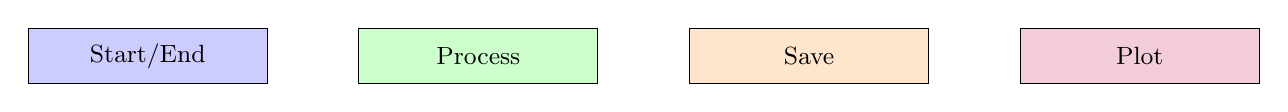
\begin{tikzpicture}[node distance=1.2cm, font=\small]
		\node[rectangle, draw, fill=blue!20, minimum height=0.7cm, text width=2.8cm, align=center] (s1) {Start/End};
		\node[rectangle, draw, fill=green!20, right of=s1, xshift=3cm, minimum height=0.7cm, text width=2.8cm, align=center] (s2) {Process};
		\node[rectangle, draw, fill=orange!20, right of=s2, xshift=3cm, minimum height=0.7cm, text width=2.8cm, align=center] (s3) {Save};
		\node[rectangle, draw, fill=purple!20, right of=s3, xshift=3cm, minimum height=0.7cm, text width=2.8cm, align=center] (s4) {Plot};
	\end{tikzpicture}
	\\[0.2cm]
	
\end{center}

\vspace{0.7cm}
\textbf{Step-by-step explanation of LSTM Model Training:}

\begin{itemize}
	\item \textbf{Start LSTM Training:} Marks the beginning of using a neural network (LSTM) for forecasting.
	\item \textbf{Extract LSTM hyperparameters:}
	\begin{itemize}
		\item Number of \textbf{epochs} – how many passes over the dataset.
		\item \textbf{Batch size} – how many samples are passed before updating weights.
		\item \textbf{Sequence length} – how many past time steps are used as input.
	\end{itemize}
	\item \textbf{Validate parameters:} Ensure chosen values are appropriate and won’t crash training or cause overfitting.
	\item \textbf{Scale wind speed data using MinMaxScaler:} LSTM needs scaled data between 0 and 1, so we normalize it.
	\item \textbf{Generate input-output sequences for LSTM:} Convert the time series into windows (X, y) for training.
	\item \textbf{Build LSTM model architecture:} Define how many layers, units, etc., the model should have.
	\item \textbf{Compile model (Adam optimizer, MSE loss):} Set the learning method and how to measure error.
	\item \textbf{Train model with validation split:} Train on a portion of data, while validating on another portion to check learning.
	\item \textbf{Save trained model and scaler:} Save both the LSTM model and the MinMaxScaler for reuse.
	\item \textbf{Forecast next 10 time steps recursively:} Use predictions as input to forecast multiple steps.
	\item \textbf{Inverse scale forecasted values:} Bring predicted values back to original range.
	\item \textbf{Save forecast CSV:} Store predictions in a CSV file.
	\item \textbf{Plot historical and forecasted wind speeds:} Visualize actual vs. predicted wind speeds.
	\item \textbf{Save plot image:} Export this plot to file.
	\item \textbf{End LSTM Training:} Complete the LSTM pipeline.
\end{itemize}

\begin{center}
	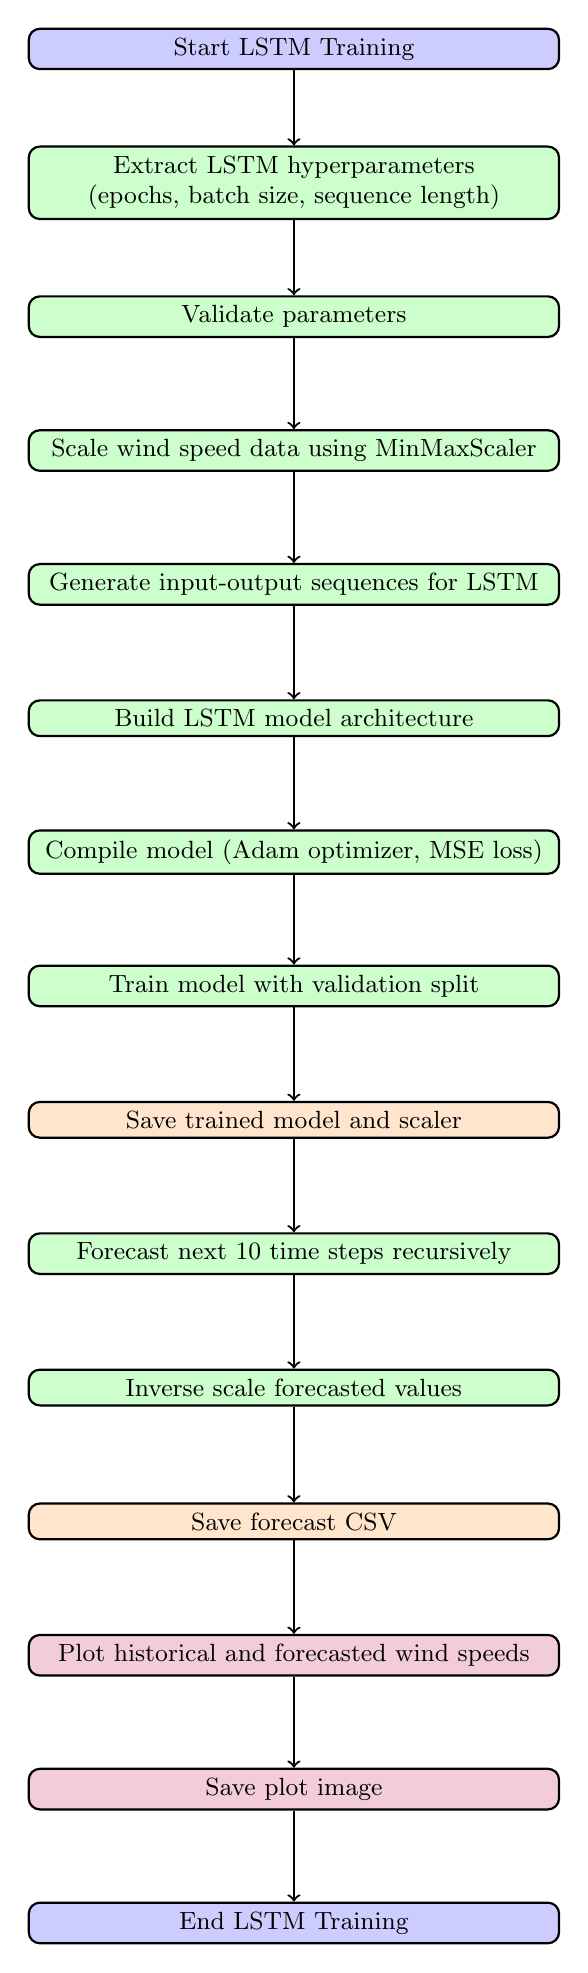
\begin{tikzpicture}[node distance=1.7cm, every node/.style={rectangle, draw, rounded corners, text width=6.5cm, align=center, font=\small}, ->, thick]
		\tikzstyle{startend} = [fill=blue!20]
		\tikzstyle{process} = [fill=green!20]
		\tikzstyle{save} = [fill=orange!20]
		\tikzstyle{plot} = [fill=purple!20]
		
		\node[startend] (start) {Start LSTM Training};
		\node[process] (extract) [below of=start] {Extract LSTM hyperparameters (epochs, batch size, sequence length)};
		\node[process] (validate) [below of=extract] {Validate parameters};
		\node[process] (scale) [below of=validate] {Scale wind speed data using MinMaxScaler};
		\node[process] (sequence) [below of=scale] {Generate input-output sequences for LSTM};
		\node[process] (build) [below of=sequence] {Build LSTM model architecture};
		\node[process] (compile) [below of=build] {Compile model (Adam optimizer, MSE loss)};
		\node[process] (train) [below of=compile] {Train model with validation split};
		\node[save] (savemodel) [below of=train] {Save trained model and scaler};
		\node[process] (forecast) [below of=savemodel] {Forecast next 10 time steps recursively};
		\node[process] (inverse) [below of=forecast] {Inverse scale forecasted values};
		\node[save] (saveforecast) [below of=inverse] {Save forecast CSV};
		\node[plot] (plot) [below of=saveforecast] {Plot historical and forecasted wind speeds};
		\node[plot] (saveplot) [below of=plot] {Save plot image};
		\node[startend] (end) [below of=saveplot] {End LSTM Training};
		
		\draw (start) -- (extract);
		\draw (extract) -- (validate);
		\draw (validate) -- (scale);
		\draw (scale) -- (sequence);
		\draw (sequence) -- (build);
		\draw (build) -- (compile);
		\draw (compile) -- (train);
		\draw (train) -- (savemodel);
		\draw (savemodel) -- (forecast);
		\draw (forecast) -- (inverse);
		\draw (inverse) -- (saveforecast);
		\draw (saveforecast) -- (plot);
		\draw (plot) -- (saveplot);
		\draw (saveplot) -- (end);
	\end{tikzpicture}
\end{center}


\section{Notation and Terminology}

In this project, we use certain words and symbols again and again. To keep things simple and clear, this section explains what they mean. Each term is written exactly the way it appears in the code or settings, along with a short and easy explanation.

\begin{description}[style=nextline,leftmargin=3.5cm]
	
	\item[\texttt{train\_data}] 
	This is the dataset we use to teach our model. It contains dates and the actual wind speed values observed in the past.
	
	\item[\texttt{forecast\_steps}] 
	The number of future time steps (like 10 days ahead) that we want the model to predict wind speeds for.
	
	\item[\(p, d, q\)] 
	These are three numbers that help the ARIMA model understand patterns in the data:
	\begin{itemize}
		\item \(p\): This tells the model how many past values (lags) it should look at. It's part of the AutoRegressive (AR) section.
		\item \(d\): This says how many times the data needs to be differenced (i.e., change it into differences) to make the trend stable. It's for removing trends and making the data stationary.
		\item \(q\): This tells the model how many past forecast errors it should consider. It's part of the Moving Average (MA) part.
	\end{itemize}
	
	\item[\texttt{sequence\_length}] 
	This is used in the LSTM model. It means how many past time steps are taken as input to predict the next value.
	
	\item[\texttt{scaler}] 
	Before training the LSTM, we scale (or normalize) the wind speed values to a range between 0 and 1 using a tool called \texttt{MinMaxScaler}. This helps the model learn better.
	
	\item[\texttt{config2.json}] 
	This is a special file in JSON format that stores all the settings (like parameters and file paths) needed to run the project. It helps us keep the setup consistent and easy to reuse.
	
	\item[\texttt{model\_choice}] 
	This is a setting where we choose which model to use. It can either be \texttt{"arima"} or \texttt{"lstm"}, depending on what kind of prediction we want.
	
	\item[\texttt{results\_csv}, \texttt{results\_png}] 
	These are the output files where we save the model's predictions. The \texttt{CSV} file stores the forecast data in a table format, and the \texttt{PNG} file saves the forecast as a plot image.
	
\end{description}

\section{Completeness of the Implementation}

Here we explain how  the current system design ensures that the training and forecasting process works reliably and can be trusted. Each part of the implementation was developed with care to make sure it runs smoothly, handles problems gracefully, and provides clear outputs. Below, we describe the key areas that make this implementation complete and reliable:

\paragraph{Data Robustness} 
One of the most important features of this system is that it can handle situations where the input data is missing or not enough. Instead of failing or crashing, the program can create synthetic (fake but realistic) data to continue working. This makes the system more robust and ensures that even if real wind speed data is not available for testing or development, the model can still be trained and evaluated without interruption.

\paragraph{Parameter Validation} 
Before the training starts, the system carefully checks if the parameters (such as the ARIMA \(p, d, q\) values or LSTM settings) are valid. If something is wrong—for example, if a number is missing or set incorrectly—the system will stop and report the problem right away. This saves time and prevents long waits for training only to discover an error later. It also reduces the chances of producing inaccurate results due to incorrect settings.

\paragraph{Modular Code Base} 
The code is neatly organized into different modules, each handling a specific part of the task. There is one module for training the ARIMA model, and another for the LSTM model. This modular design makes the code easier to read, test, and maintain. For example, if we only want to change how LSTM works, we can do that without touching the ARIMA code. It also helps new users understand and navigate the code quickly.

\paragraph{Output Artifacts} 
Each time the model is trained, the system saves important files like:
\begin{itemize}
	\item the trained model itself (so we can reuse it later),
	\item the forecast values in a CSV file (which is like a table), and
	\item a plot image that shows both the real and predicted wind speeds.
\end{itemize}
These outputs make the process transparent and reproducible, which means anyone can check the results or run the same experiment again and expect the same output.

\paragraph{Logging and Error Handling} 
As the system runs, it prints out clear messages explaining what it is doing—whether it’s loading data, training the model, saving files, or encountering errors. This logging is very helpful for developers and users because it makes the process easier to follow and speeds up troubleshooting when something goes wrong. Error handling also ensures the program exits gracefully without crashing.

\paragraph{Configurability} 
All the important settings—like model type, number of epochs, or where to save files—are stored in a single \texttt{config2.json} file. This means that users can try new settings or tweak experiments just by editing that one file, without needing to touch the main Python code. This makes the system flexible and beginner-friendly for testing different ideas or running new experiments.


\section{Machine Learning Pipeline Details}

The machine learning pipeline used in this project is designed to process raw wind speed data and produce accurate, meaningful forecasts. The pipeline handles both ARIMA and LSTM models. Below is a step-by-step explanation of each stage, aimed at beginners, accompanied by a TikZ diagram.

\subsection*{Step-by-Step Description}

\begin{description}[style=nextline,leftmargin=1.5cm]
	\item[\textbf{1. Data Ingestion}]
	This is the first step where the program loads the wind speed dataset. If the real dataset is missing or not enough, it creates a small fake (synthetic) dataset to keep things running. This ensures that the code never crashes due to missing input.
	\item[\textbf{2. Data Preprocessing}]
	In this stage, the data is arranged in the correct time order (chronological). Any missing values are filled using techniques like forward fill or interpolation. The program also prepares the data so that it can be easily given to the model (like making sure it has only the needed columns).
	
	\item[\textbf{3. Feature Scaling (LSTM only)}]
	LSTM models work better when the numbers are small and consistent. So here, all wind speed values are converted into a range between 0 and 1 using MinMaxScaler. This helps the model learn faster and prevents big numbers from dominating the learning process.
	
	\item[\textbf{4. Sequence Generation (LSTM only)}]
	Because LSTM looks at patterns over time, the data must be converted into small overlapping parts. For example, if the sequence length is 3, the model will look at 3 past days to predict the next one. This creates input-output pairs that the model can learn from.
	
	\item[\textbf{5. Model Training}]
	This is where the model actually learns from the data. For ARIMA, it fits a mathematical formula using the (p, d, q) values. For LSTM, it uses deep learning and trains the model for multiple rounds (called epochs) with the data sequences.
	
	\item[\textbf{6. Model Validation (LSTM)}]
	During training, the LSTM model checks its accuracy on a small portion of data that it did not train on. This helps to make sure the model is not just memorizing data but is truly learning. If the model does well here, it usually performs well on unseen data too.
	
	\item[\textbf{7. Forecasting}]
	After training, the model is asked to predict future wind speeds. It does this for a fixed number of steps (e.g., the next 10 hours or days). This step is key for planning and decision-making.
	
	\item[\textbf{8. Post-processing}]
	For LSTM, the predictions made in step 7 are still in the 0 to 1 range (scaled form). So they need to be converted back to the real wind speed values using inverse scaling. This makes the results understandable and usable.
	
	\item[\textbf{9. Output Saving}]
	Finally, the program saves everything---the trained model, the forecasts (in a CSV file), and the plots (as PNG images). These files can be used for reports or for loading the model later without training again.
\end{description}

\subsection{ ML Pipeline Overview-Diagram}

\begin{center}
	\begin{tikzpicture}[node distance=1.4cm and 2.2cm, 
		every node/.style={rectangle, draw, rounded corners=4pt, fill=blue!5, text width=5cm, align=center, font=\small}, 
		>=latex']
		
		\node (ingest) {\textbf{Data Ingestion}\\Load wind speed data or generate synthetic data};
		\node (preprocess) [below=of ingest] {\textbf{Data Preprocessing}\\Sort, fill missing values, clean data};
		\node (scale) [below=of preprocess] {\textbf{Feature Scaling (LSTM)}\\Normalize data using MinMaxScaler};
		\node (sequence) [below=of scale] {\textbf{Sequence Generation (LSTM)}\\Create overlapping sequences};
		\node (train) [below=of sequence] {\textbf{Model Training}\\Train ARIMA or LSTM model};
		\node (validate) [below=of train] {\textbf{Model Validation (LSTM)}\\Check overfitting using validation data};
		\node (forecast) [below=of validate] {\textbf{Forecasting}\\Predict next 10 time steps};
		\node (postprocess) [below=of forecast] {\textbf{Post-processing (LSTM)}\\Inverse scale to real values};
		\node (save) [below=of postprocess] {\textbf{Output Saving}\\Save models, forecasts, plots};
		
		\draw[->] (ingest) -- (preprocess);
		\draw[->] (preprocess) -- (scale);
		\draw[->] (scale) -- (sequence);
		\draw[->] (sequence) -- (train);
		\draw[->] (train) -- (validate);
		\draw[->] (validate) -- (forecast);
		\draw[->] (forecast) -- (postprocess);
		\draw[->] (postprocess) -- (save);
		
	\end{tikzpicture}
\end{center}


\subsection*{Legend}
\begin{itemize}
\item \textbf{Blue Boxes}: Represent each logical stage in the ML pipeline.
\item \textbf{Arrows}: Show the flow of processing from one step to the next.
\item \textbf{LSTM Only Steps}: Steps 3, 4, 6, and 8 apply only to the LSTM model.
\end{itemize}

This structured pipeline ensures that data flows smoothly from raw input to usable output, while also being flexible enough to switch between ARIMA and LSTM depending on the configuration.

\section{Program Readability and Coding Practices}

Good coding practices and clear organization are crucial for writing software that is easy to understand, maintain, and extend. In this project, the code is divided into well-defined modules, each responsible for a specific part of the machine learning workflow. This makes it easier for developers to work on different parts without conflicts and to find code quickly.

\subsection{Project Structure and Modularization Explained}

\begin{table}[h!]
	\centering
	\begin{tabular}{|p{3cm}|p{7cm}|p{4.5cm}|}
		\hline
		\textbf{Module Name} & \textbf{Responsibility} & \textbf{Benefits} \\ \hline
		
		\texttt{train\_models.py} &
		Main control script that reads user settings, loads data, selects which model (ARIMA or LSTM) to train, and manages the training workflow. &
		Acts as the “brain” organizing the pipeline; allows running the program with different options easily. \\ \hline
		
		\texttt{arima\_train.py} &
		Contains functions for ARIMA: parameter validation, fitting the model, forecasting, and saving results. &
		Isolates ARIMA logic, simplifies debugging and maintenance of ARIMA-specific code. \\ \hline
		
		\texttt{lstm\_train.py} &
		Handles LSTM-specific preprocessing, model architecture, training, forecasting, and saving outputs. &
		Separates LSTM complexity for focused development and debugging of deep learning parts. \\ \hline
		
		\texttt{utils.py} &
		Provides shared utility functions like data validation, plotting, file management, and logging used across modules. &
		Avoids code duplication and improves overall code readability and maintainability. \\ \hline
		
	\end{tabular}
	\caption{Project Modules and Their Responsibilities}
\end{table}

\subsection{Why Modularization Matters (Simple Explanation)}

\begin{itemize}
	\item \textbf{Easier to understand:} Smaller, focused modules let developers concentrate on one topic at a time.
	\item \textbf{Simplifies debugging:} Problems can be isolated quickly to a specific module rather than searching the entire codebase.
	\item \textbf{Encourages teamwork:} Different developers can work simultaneously on separate modules without conflicts.
	\item \textbf{Facilitates reusability:} Utility functions in \texttt{utils.py} are shared across modules, reducing redundancy.
\end{itemize}

\subsection{Visualizing the Project Structure}



\begin{center}
	\resizebox{\textwidth}{!}{ % scale horizontally to text width, keep aspect ratio
		\begin{tikzpicture}[
			module/.style={
				rectangle, draw=black, thick, fill=blue!10, 
				rounded corners, minimum width=3.8cm, minimum height=1.2cm, 
				font=\footnotesize, align=center},
			arrow/.style={thick, ->, >=stealth}
			]
			
			% Nodes
			\node[module] (train) {train\_models.py\\\footnotesize Main control and orchestration};
			\node[module, below left=1.4cm and 1.4cm of train] (arima) {arima\_train.py\\\footnotesize ARIMA-specific training and forecasting};
			\node[module, below right=1.4cm and 1.4cm of train] (lstm) {lstm\_train.py\\\footnotesize LSTM-specific preprocessing and training};
			\node[module, below=2.8cm of train] (utils) {utils.py\\\footnotesize Shared utility functions};
			
			% Arrows
			\draw[arrow] (train) -- (arima);
			\draw[arrow] (train) -- (lstm);
			\draw[arrow] (train) -- (utils);
			\draw[arrow] (arima) -- (utils);
			\draw[arrow] (lstm) -- (utils);
			
		\end{tikzpicture}
	}
\end{center}




Above diagram shows how the main script controls the two model-specific modules, and how both rely on shared utility functions. This clear separation ensures easy maintenance, teamwork, and scalability.


\subsection{Parameter Handling}

Effective parameter handling is critical for making the codebase flexible, robust, and easy to maintain. In our project, all model hyperparameters and file paths are centrally managed through the external configuration file \texttt{config2.json}. This approach enables:

\begin{itemize}
	\item \textbf{Reproducibility:} The exact training conditions can be saved, shared, and reloaded easily.
	\item \textbf{Ease of Experimentation:} Changing model parameters or file locations does not require code edits, just updating the config file.
\end{itemize}

To ensure robustness, the system performs rigorous validation of these parameters before training starts. This includes checking:

\begin{itemize}
	\item \textbf{Presence:} Mandatory parameters must be present.
	\item \textbf{Type:} Each parameter is validated against its expected data type (e.g., integers, floats, strings).
	\item \textbf{Value ranges:} Numeric parameters are checked to lie within acceptable bounds (e.g., learning rate between 0 and 1).
\end{itemize}

Fallback default values are defined in the code for optional parameters to maintain resilience if some entries are missing from the config file.

If any parameter fails validation, the system immediately raises a descriptive error with details on the invalid parameter and expected values. This early failure prevents wasted compute time and reduces debugging efforts.

\vspace{0.5em}
\noindent





\begin{figure}[H]
	\centering
	\begin{tikzpicture}[nodes in empty cells,
		table/.style={
			rectangle, draw=black, thick, rounded corners,
			minimum height=1.6cm, font=\small, align=left, inner sep=10pt
		},
		header/.style={table, fill=gray!30, align=center, font=\bfseries},
		col1/.style={table, fill=blue!20, align=center, text width=5.5cm},
		col2/.style={table, fill=blue!10, text width=7cm},
		col3/.style={table, fill=blue!5, text width=9cm},
		row sep=10mm,
		column sep=18mm
		]
		\matrix (m) [matrix of nodes, row sep=10mm, column sep=18mm,
		nodes={table, anchor=center, text depth=0.25ex}] {
			\node[header] {Check}; & \node[header] {Purpose}; & \node[header] {Example}; \\
			\node[col1] {Presence}; & \node[col2] {Ensure required parameters exist}; & \node[col3] {\texttt{Check if "learning\_rate" key exists in config2.json}}; \\
			\node[col1] {Type}; & \node[col2] {Confirm parameter type correctness}; & \node[col3] {\texttt{Verify "batch\_size" is an integer}}; \\
			\node[col1] {Range}; & \node[col2] {Confirm numeric values are valid}; & \node[col3] {\texttt{Check "dropout" is in [0, 1]}}; \\
			\node[col1] {Defaults}; & \node[col2] {Use predefined fallback values}; & \node[col3] {Use 0.01 as default learning rate if missing}; \\
			\node[col1] {Error Reporting}; & \node[col2] {Raise clear, descriptive exceptions}; & \node[col3] {\texttt{"Parameter dropout must be between 0 and 1"}}; \\
		};
	\end{tikzpicture}
	\caption{Validation checks during configuration parsing}
	\label{fig:config-checks}
\end{figure}



\subsection{Error Handling and Messaging}

Robust error handling is vital for maintaining stable training workflows and simplifying debugging. Our approach involves structured try-except blocks wrapping all critical operations such as:

\begin{itemize}
	\item Reading input data files.
	\item Fitting ARIMA or LSTM models.
	\item Saving trained model artifacts and forecasts.
\end{itemize}

Whenever an exception occurs, it is:

\begin{itemize}
	\item Logged with a detailed stack trace for developer diagnosis.
	\item Accompanied by a clear, user-friendly message indicating what went wrong.
\end{itemize}

Conversely, successful milestones (e.g., ``LSTM model trained successfully'') generate informational logs to provide progress visibility.

This structured messaging system drastically reduces time lost on silent failures or vague error reports.

\vspace{1em}


\begin{center}
	\begin{tikzpicture}[
		node distance=1.8cm and 3.5cm,
		startstop/.style={
			rectangle, rounded corners, draw, fill=red!20,
			minimum width=4cm, minimum height=1cm,
			text centered, font=\small,
			align=center
		},
		process/.style={
			rectangle, draw, fill=blue!20,
			minimum width=4cm, minimum height=1cm,
			text centered, font=\small,
			align=center
		},
		decision/.style={
			diamond, draw, fill=yellow!20,
			minimum width=4cm, minimum height=1cm,
			text centered, font=\small,
			aspect=2,
			align=center
		},
		arrow/.style={thick,->,>=Stealth}
		]
		
		% Nodes
		\node[startstop] (start) {Start Critical Operation};
		\node[process] (tryblock) at ([yshift=-1.8cm]start.south) {Try Block Executes};
		\node[decision] (errorcheck) at ([yshift=-1.8cm]tryblock.south) {Error Occurred?};
		\node[process] (handleerror) at ([xshift=3.5cm]errorcheck.east) {Log Error with Stack Trace\\Show User-Friendly Message};
		\node[process] (success) at ([yshift=-1.8cm]errorcheck.south) {Log Success Message};
		\node[startstop] (end) at ([yshift=-1.8cm]success.south) {Operation Ends};
		
		% Arrows
		\draw[arrow] (start) -- (tryblock);
		\draw[arrow] (tryblock) -- (errorcheck);
		\draw[arrow] (errorcheck) -- node[above] {Yes} (handleerror);
		\draw[arrow] (handleerror) |- (end);
		\draw[arrow] (errorcheck) -- node[right] {No} (success);
		\draw[arrow] (success) -- (end);
	\end{tikzpicture}
\end{center}

	



\section{Future Work and Improvements}

\begin{itemize}
	\item \textbf{Model Expansion}: Incorporate additional forecasting algorithms such as Prophet, XGBoost, or hybrid ensemble models.
	\item \textbf{Data Augmentation}: Integrate external meteorological features (pressure, humidity) to improve model accuracy.
	\item \textbf{Hyperparameter Tuning}: Automate hyperparameter search using grid search or Bayesian optimization.
	\item \textbf{Continuous Integration}: Implement automated testing and deployment pipelines for faster iteration.
	\item \textbf{Visualization Enhancements}: Develop interactive dashboards with Streamlit or Dash for real-time forecast visualization.
\end{itemize}

\subsection{Project File Structure: \texttt{hurricane\_predictor\_ready}}

The main components of the project folder \texttt{hurricane\_predictor\_ready}, detailing the organization of files, modules, functions, and key variables used throughout the application.

\begin{itemize}
	\item \textbf{Main File:}
	\begin{itemize}
		\item \texttt{app.py} – Entry point of the Streamlit web application.
	\end{itemize}
	
	\item \textbf{Folders:}
	\begin{itemize}
		\item \texttt{models/} – Contains serialized ARIMA and LSTM models.
		\item \texttt{data/} – Stores input CSV files used for prediction.
		\item \texttt{plots/} – Saves output images and visualizations.
		\item \texttt{utils/} – Holds reusable modules for preprocessing and forecasting.
	\end{itemize}
	
	\item \textbf{Files:}
	\begin{itemize}
		\item \texttt{ARIMA.py} – Implements ARIMA model logic.
		\item \texttt{LSTM.py} – Contains the LSTM training and prediction code.
		\item \texttt{preprocessing.py} – Data cleaning, formatting, and splitting.
		\item \texttt{config.py} – Centralized file for model parameters and settings.
	\end{itemize}
	
	\item \textbf{Modules:}
	\begin{itemize}
		\item \texttt{pandas, numpy, matplotlib, seaborn} – For data handling and plotting.
		\item \texttt{statsmodels, keras, sklearn} – For model implementation and evaluation.
		\item \texttt{streamlit} – For building the user interface.
	\end{itemize}
	
	\item \textbf{Functions:}
	\begin{itemize}
		\item \texttt{train\_arima(data, p, d, q)} – Fits the ARIMA model.
		\item \texttt{train\_lstm(X, y, epochs, batch\_size)} – Builds and trains the LSTM.
		\item \texttt{make\_forecast(model, input)} – Performs prediction using trained model.
		\item \texttt{visualize\_forecast(y\_true, y\_pred)} – Generates output plots.
	\end{itemize}
	
	\item \textbf{Variables:}
	\begin{itemize}
		\item \texttt{wind\_speed} – Main time series feature.
		\item \texttt{date} – Date/time column for indexing.
		\item \texttt{forecast\_results} – Stores model predictions for output.
		\item \texttt{arima\_model, lstm\_model} – Trained model objects.
	\end{itemize}
\end{itemize}




	








